% hack to deal with beamer/pgf bug
\RequirePackage{atbegshi}

% "draft" makes compilation faster; remove for final version
% shadow = put drop shadows behind blocks by default
% xcolor: svgnames imports lots of color names
% table allows for multi-color table rows
% pdftex is the compiler
\documentclass[shadow,xcolor=pdftex,svgnames,table,t]{beamer}

\usepackage{amsmath,amssymb,amsfonts}

% need to load tikz defs before beamer defs, for some reason
\input{tikzhead}
%% BOILERPLATE PRESENTATION STUFF

% an underlining package
\usepackage{ulem}
% use normal italics for emphasis
\normalem


% dingbats
\usepackage{pifont}

\renewcommand{\Check}{\ding{52}}
\newcommand{\Cross}{\ding{55}}
\newcommand{\Hand}{\ding{43}}
\newcommand{\GreenCheck}{{\textcolor{green}\Check}}
\newcommand{\RedCross}{{\textcolor{red}\Cross}}

% alias for citations
\newcommand{\citationsize}{\footnotesize}

\subject{Theoretical Computer Science}

% suppress ugly QEDs in proofs
\def\qedsymbol{}


% common stuff
% basic notation

\newcommand{\lamperp}{\Lambda^{\perp}}
\newcommand{\lam}{\Lambda}

% lattice
\newcommand{\lat}{\mathcal{L}}
% fundamental region
\newcommand{\piped}{\mathcal{P}}
% smoothing parameter
\newcommand{\smooth}{\eta}
% smoothing w/ epsilon
\newcommand{\smootheps}{\smooth_{\epsilon}}
% ball
\newcommand{\ball}{\mathcal{B}}
% cube
\newcommand{\cube}{\mathcal{C}}
% covering radius symbol
\newcommand{\cover}{\ensuremath{\mu}}
% Gram-Schmidt
\newcommand{\gs}[1]{\ensuremath{\widetilde{#1}}}
% GS minimum
\newcommand{\gsmin}{\ensuremath{\tilde{bl}}}
% volume operation
\DeclareMathOperator{\vol}{vol}
% Hermite normal form
\DeclareMathOperator{\hnf}{HNF}
% rank
\DeclareMathOperator{\rank}{rank}
% distance operator
\DeclareMathOperator{\dist}{dist}
% span operator
\DeclareMathOperator{\spn}{span}
% error function
\DeclareMathOperator{\erf}{erf}

% quantities that show up regularly
\newcommand{\wsln}{\ensuremath{\omega(\sqrt{\log n})}}
\newcommand{\wslm}{\ensuremath{\omega(\sqrt{\log m})}}

% support algorithms
\newcommand{\sampleZ}{\algo{Sample}\Z}
\newcommand{\sampleD}{\algo{SampleD}}
\newcommand{\tobasis}{\algo{ToBasis}}
\newcommand{\invert}{\algo{Invert}}
\newcommand{\genbasis}{\algo{GenBasis}}
\newcommand{\extbasis}{\algo{ExtBasis}}
\newcommand{\extlattice}{\algo{ExtLattice}}
\newcommand{\randbasis}{\algo{RandBasis}}
\newcommand{\gentrap}{\algo{GenTrap}}
\newcommand{\deltrap}{\algo{DelTrap}}
\newcommand{\noisy}{\algo{Noisy}}

% problems related to lattices
\newcommand{\svp}{\problem{SVP}}
\newcommand{\gapsvp}{\problem{GapSVP}}
\newcommand{\cogapsvp}{\problem{coGapSVP}}
\newcommand{\usvp}{\problem{uSVP}}
\newcommand{\sivp}{\problem{SIVP}}
\newcommand{\gapsivp}{\problem{GapSIVP}}
\newcommand{\cvp}{\problem{CVP}}
\newcommand{\gapcvp}{\problem{GapCVP}}
\newcommand{\cvpp}{\problem{CVPP}}
\newcommand{\gapcvpp}{\problem{GapCVPP}}
\newcommand{\bdd}{\problem{BDD}}
\newcommand{\gdd}{\problem{GDD}}
\newcommand{\add}{\problem{ADD}}
\newcommand{\incgdd}{\problem{IncGDD}}
\newcommand{\incivd}{\problem{IncIVD}}
\newcommand{\crp}{\problem{CRP}}
\newcommand{\gapcrp}{\problem{GapCRP}}
% problems on ideal lattices
\newcommand{\igvp}{\problem{IGVP}}
\newcommand{\incigvp}{\problem{IncIGVP}}
% avg-case stuff
\newcommand{\sis}{\problem{SIS}}
\newcommand{\isis}{\problem{ISIS}}
\newcommand{\ilwe}{\problem{ILWE}}
\newcommand{\lwe}{\problem{LWE}}
\newcommand{\rlwe}{\problem{RLWE}}
\newcommand{\lwr}{\problem{LWR}}
\newcommand{\rlwr}{\problem{RLWR}}
\newcommand{\dlwe}{\problem{DLWE}}
\newcommand{\lpn}{\problem{LPN}}
\newcommand{\Psibar}{\ensuremath{\bar{\Psi}}}

\newcommand{\extlwe}{\problem{Ext \text{\textendash} LWE}}
\newcommand{\extrlwe}{\problem{Ext \text{\textendash} RLWE}}

% Module-LWE and variants
\newcommand{\mlwe}{\problem{M \text{\textendash} LWE}}
\newcommand{\extmlwe}{\problem{Ext \text{\textendash}  M \text{\textendash} LWE}}
\newcommand{\mlwr}{\problem{M \text{\textendash}  LWR}}
\input{../vecmathead}
% "left-right" pairs of symbols

\usepackage{mathtools}

% inner product
\DeclarePairedDelimiter\inner{\langle}{\rangle}
% absolute value
\DeclarePairedDelimiter\abs{\lvert}{\rvert}
% a set
\DeclarePairedDelimiter\set{\{}{\}}
% parens
\DeclarePairedDelimiter\parens{(}{)}
% tuple, alias for parens
\DeclarePairedDelimiter\tuple{(}{)}
% square brackets
\DeclarePairedDelimiter\bracks{[}{]}
% rounding off
\DeclarePairedDelimiter\round{\lfloor}{\rceil}
% floor function
\DeclarePairedDelimiter\floor{\lfloor}{\rfloor}
% ceiling function
\DeclarePairedDelimiter\ceil{\lceil}{\rceil}
% length of some vector, element
\DeclarePairedDelimiter\length{\lVert}{\rVert}
% "lifting" of a residue class
\DeclarePairedDelimiter\lift{\llbracket}{\rrbracket}

\input{../bbhead}

% restricts presentation to specified frames, for faster compilation;
% comment out the line to get the entire presentation

% \includeonlyframes{hibe}

\begin{document}

\begin{frame}{Bootstrapping}
  \begin{itemize}
    \vfill
  \item ``Bootstrapping'' {\footnotesize [Gen'09]} homomorphically
    evaluates a decryption circuit to ``refresh'' a ciphertext (i.e.,
    reduce the noise) for further homom evaluation.

    \begin{itemize}
    \item \alert{Essential} to \alert{unbounded} FHE.

      \medskip
    \item \uline{Need}: minimize (multiplicative) \alert{depth} and
      \alert{size} of decryption circuit.

      Yields a faster, more secure FHE scheme.
    \end{itemize}

    \vfill

  \item Intensive study, many techniques {\footnotesize
      [G'09,GH'11a,GH'11b,GHS'12a,GHS'12b]}, but is still inefficient
    and quite complex
    \medskip

    \begin{itemize}
    \item $O(\log n)$ depth, but the hidden constant matters -- a lot!
    \end{itemize}

    \medskip 
  
  \item The (theoretically) most efficient methods on ``packed''
    ciphertexts {\footnotesize [GHS'12a,GHS'12b]} seem very hard to
    implement
    \vfill
  \end{itemize}
\end{frame}

\begin{frame}{Simple, Efficient Bootstrapping: Main Ideas}
  \begin{itemize}
  \item Lattice-based decryption $\text{Dec} \colon \Z^{n} \times
    \Zq^{n} \to \Z_{2}$ works in two steps.

    \medskip
    On input $(\vecs, \vecc)$:

    \begin{enumerate}
    \item Compute $d = \inner{\vecs, \vecc} \in \Zq$. \hfill (Linear,
      trivial homomorphically.)

      \medskip
    \item ``Round'' to $\text{msb}(d) := [d \approx \frac{q}{2}] \in
      \Z_{2}$.\hfill (\alert{Non-linear, expensive homom'ly.})
    \end{enumerate}

    \smallskip
    Note: $\text{Dec}$ is run on ``reduced'' ciphertexts: $n$ small, $q
    \approx \sqrt{n}$.
  \end{itemize}

  \uline{Advances}:
  \begin{enumerate}
  \item A very \alert{simple}, \alert{low-depth} rounding circuit for
    $q=2^{k}$.

    \begin{itemize}
    \item Depth exactly $\log_{2}(q/2)$, exactly $(q/2-1)$ mults, no adds.
      \smallskip
    \item Best exact depth and circuit size -- by quite a bit.
    \end{itemize}

    \medskip
  \item Additional techniques for ``\alert{packed}'' ciphertexts in
    polynomial rings.

    \begin{itemize}
    \item Fast homomorphic extraction of polynomial coefficients:
      \[ a(X) = \sum_{i} a_{i} X^{i} \in R_{q} \quad \longrightarrow \quad
      a_{i} \in \Z_{q} \]
    \end{itemize}
  \end{enumerate}
\end{frame}

\begin{frame}{Rounding $\Zq$ to $\Z_{2}$}
  \begin{itemize}
  \item Example: round $d \in \Z_{8}$ to $\text{msb}(d) \in \Z_{2}$ with
    an arithmetic formula
  \end{itemize}

  \begin{center}
    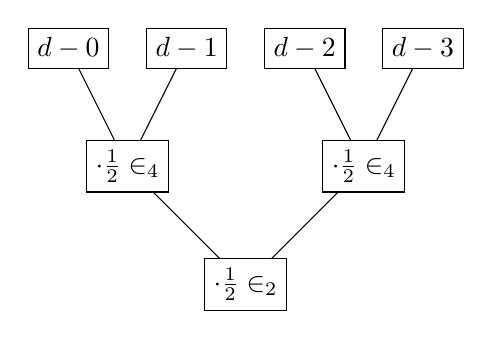
\begin{tikzpicture}[every node/.style=draw,
      level 1/.style={draw,sibling distance=3cm},
      level 2/.style={draw,sibling distance=1.5cm},
      level 3/.style={sibling distance=0.75cm}]
      \node {$\cdot \frac12 \in \Z_{2}$} [grow'=up]
      child { node {$\cdot \frac12 \in \Z_{4}$}
        child {node {$d-0$}}
        child {node {$d-1$}}
      }
      child {node {$\cdot \frac12 \in \Z_{4}$}
        child {node {$d-2$}}
        child {node {$d-3$}}
      }
      ;
    \end{tikzpicture}
  \end{center}

  \begin{itemize}
  \item[] (Homomorphic mult-by-$\frac12$ is a null op.)

    \medskip
  \item In general: $q-1$ mults in a $\log_{2}(q/2)$-depth binary tree
  \end{itemize}
\end{frame}

\begin{frame}[c]{Extracting Coefficients, Homomorphically}
  \begin{center}
    \begin{tikzpicture}
      \node (K) at (0,0) {$K=\Q(\zeta_{m},\zeta_{m'})$};
      \node (K0) at (-3,-3) {$K_{0}=\Q(\zeta_{m})$};
      \node (K1) at (3,-3) {$K_{1} = \Q(\zeta_{m'})$};
      \node (Q) at (0,-6) {$\Q$};

      \path[->] (K0) edge node[above,sloped] {embed $ct$} (K)
      (K) edge node[above,sloped] {$\text{Trace}_{K/K_{1}}$} (K1)
      (K0) edge node[above,sloped] {$\text{Trace}_{K_{0}/\Q}$} (Q)
      ;
    \end{tikzpicture}
  \end{center}
\end{frame}

\end{document}

%%% Local Variables: 
%%% mode: latex
%%% TeX-master: t
%%% End: 
